% !TEX root = ../main.tex
\chapter{Student Workshop Activity \& Worksheets}

\section{Activity 1: LED Indicator Breadboard Assembly \& Circuit Calculations}

\subsection{Objective \& Theoretical Parameter Calculations}
The objective of this laboratory exercise is to design, calculate, assemble, and quantitatively verify a current-limited LED indicator circuit on a solderless breadboard.

Given a regulated DC source voltage $V_{CC} = 5.0\text{ V}$, a standard indicator LED has a typical forward voltage drop $V_F \approx 2.0\text{ V}$ and a target forward current $I_F \approx 9.1\text{ mA}$ ($0.0091\text{ A}$). Applying Kirchhoff's Voltage Law (KVL) and Ohm's Law across the series loop:

\begin{equation}
    V_{CC} = V_R + V_F \implies V_R = V_{CC} - V_F
\end{equation}
\begin{equation}
    R = \frac{V_{CC} - V_F}{I_F} = \frac{5.0\text{ V} - 2.0\text{ V}}{0.0091\text{ A}} \approx 330\ \Omega
\end{equation}

Thus, a standard $330\ \Omega$ ($1/4\text{ W}$) resistor provides optimal current limiting, preventing thermal runaway and catastrophic semiconductor burnout.

\begin{figure}[htbp]
    \centering
    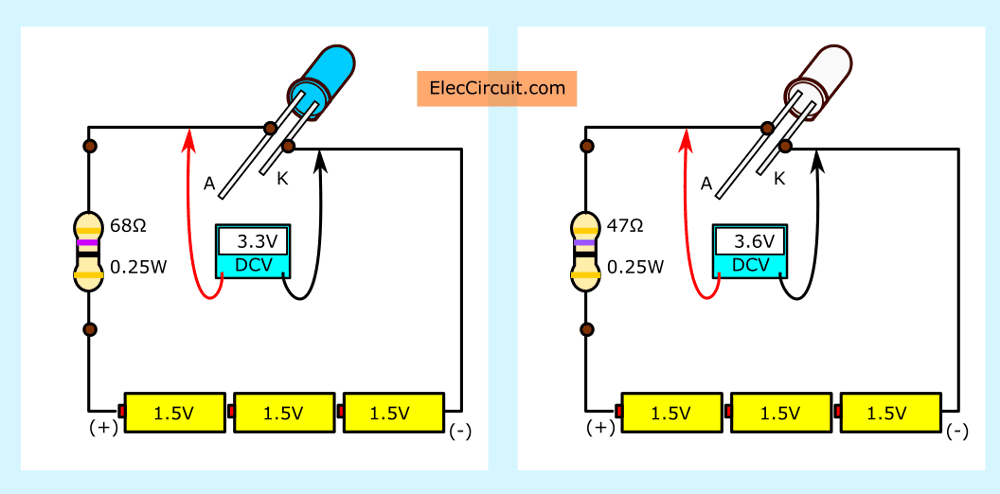
\includegraphics[width=0.88\textwidth]{figures/fig_led_schematic_wiring.png}
    \caption{Series LED indicator circuit schematic and Digital Multimeter (DMM) DC voltage probe verification across LED terminals ($A$ to $K$) using series current-limiting resistors \cite{eleccircuit_leds}.}
    \label{fig:led_schematic_wiring}
\end{figure}
\subsection{Step-by-Step Breadboard Assembly Protocol}
\begin{activitybox}
\textbf{ASSEMBLY PROTOCOL:}
\begin{enumerate}[leftmargin=1.5em]
    \item \textbf{Bench Power Configuration:} Turn on the DC power supply with output leads disconnected from the breadboard. Adjust the output to exactly $5.0\text{ V}$. Set the current limit knob to approximately mid-scale ($500\text{ mA}$). Turn the supply output switch OFF before connecting leads to the breadboard.
    \item \textbf{Rail Connections:} Connect the red power lead to the breadboard positive ($+$) bus and the black lead to the negative ($-$/GND) bus.
    \item \textbf{Resistor Placement:} Insert one lead of the $330\ \Omega$ resistor into the positive ($+$) rail and the other lead into terminal Row 10.
    \item \textbf{LED Insertion:} Identify the LED polarity: the longer lead is the \textbf{anode} ($+$) and the shorter lead with the flat cathode rim is the \textbf{cathode} ($-$). Insert the anode into terminal Row 10 (sharing the spring clip with the resistor) and the cathode into the negative ground rail.
    \item \textbf{Power Verification:} Energize the DC output. The LED will illuminate. Using a DMM set to DC Volts, verify approximately $5.0\text{ V}$ across the rails, $3.0\text{ V}$ across the resistor, and $2.0\text{ V}$ across the LED.
\end{enumerate}
\end{activitybox}

\section{Activity 2: Hands-On Demonstration --- Introduction to Soldering}

\subsection{Soldering Station Setup \& Temperature Calibration}
Soldering creates permanent electrical joints and mechanical bonds using an alloy filler metal.
\begin{itemize}[leftmargin=1.5em]
    \item \textbf{Personal Protective Equipment (PPE):} Safety glasses are mandatory. Ensure the local fume extractor is active.
    \item \textbf{Temperature Setting:} Set the soldering station to approximately \textbf{350\textdegree C (660\textdegree F)} for standard lead-free alloy solder wire. Allow 1--2 minutes for thermal equilibrium.
    \item \textbf{The Golden Rule:} Return the soldering iron to its safety stand the moment it leaves your hand. Never rest a hot iron on the bench surface.
\end{itemize}

\subsection{Tip Maintenance, Tinning, and Joint Formation}
\begin{enumerate}[leftmargin=1.5em]
    \item \textbf{Tip Cleaning \& Tinning:} Wipe the hot tip against a damp brass wire sponge or moist cellulose sponge. Immediately apply a small bead of fresh solder to the tip (tinning). This prevents oxidation and ensures rapid thermal conduction.
    \item \textbf{Heating the Joint:} Position the iron chisel tip so it makes simultaneous contact with both the copper PCB pad and the component lead. Hold for approximately 2 seconds to bring both surfaces up to soldering temperature.
    \item \textbf{Feeding Solder:} Introduce solder wire directly to the \textbf{heated joint} (not to the iron tip itself). The solder will melt, flow smoothly, and wet both surfaces.
    \item \textbf{Cooling:} Withdraw the solder wire first, followed immediately by the iron tip. Allow the joint to cool undisturbed for 3 seconds.
\end{enumerate}

\begin{figure}[htbp]
    \centering
    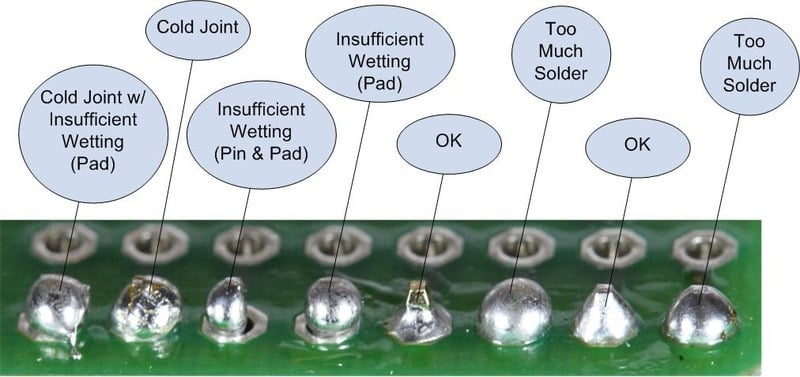
\includegraphics[width=0.88\textwidth]{figures/fig_solder_joints.jpg}
    \caption{Visual inspection criteria of PCB through-hole solder connections: distinguishing acceptable concave fillets (``OK'') from defective cold joints, insufficient pad/pin wetting, and excessive solder buildup \cite{adafruit_soldering_guide}.}
    \label{fig:solder_joints}
\end{figure}

\subsection{Joint Inspection Criteria}
\begin{itemize}[leftmargin=1.5em]
    \item \textbf{Acceptable Joint:} Features a shiny, smooth surface with a concave fillet (resembling a miniature tent or volcano) wetting both the lead and pad.
    \item \textbf{Defective Cold Joint:} Appears dull, grainy, or forms a spherical bead without wetting. To rework: reapply tip heat with a touch of flux-core solder for 2--3 seconds until reflow occurs.
    \item \textbf{Lead Trimming:} Trim excess component leads flush with the top of the solder fillet using flush wire cutters.
\end{itemize}
